%!TEX root =  ./JanasJanssenCuffaro-August2019.tex

%SUBSECTION 2.6
\subsection{The elliptope and the geometry of correlations} \label{1.6}

In Section \ref{1.5} we derived the equation for the elliptope using elements of quantum mechanics. In particular, we used the Born rule to show that the anti-correlation coefficients $(\chi_{ab}, \chi_{ac}, \chi_{bc})$ in the Mermin setup are given by the cosines of the angles $(\varphi_{ab}, \varphi_{ac}, \varphi_{bc})$ between the peeling directions $(\vec{e}_a, \vec{e}_b, \vec{e}_c)$. That meant that the anti-correlation matrix $\chi$ is a Gram matrix:
\begin{equation}
\chi \equiv \begin{pmatrix}
1 & \chi_{ab} & \chi_{ac} \\[.2 cm]
\chi_{ab} & 1 & \chi_{bc} \\[.2 cm]
\chi_{ac} & \chi_{bc} & 1
\end{pmatrix} =
\begin{pmatrix}
\vec{e}_a \!  \cdot  \vec{e}_a &  \vec{e}_a \! \cdot  \vec{e}_b  &   \vec{e}_a \! \cdot  \vec{e}_c  \\[.2cm]
\vec{e}_b \!  \cdot  \vec{e}_a & \vec{e}_b \! \cdot  \vec{e}_b & \vec{e}_b \! \cdot  \vec{e}_c \\[.2cm]
\vec{e}_c \!  \cdot   \vec{e}_a & \vec{e}_c \! \cdot  \vec{e}_b  & \vec{e}_c \! \cdot  \vec{e}_c 
\end{pmatrix}.
\label{gram matrix reprise}
\end{equation}
Eq.\ (\ref{QM14}) for the elliptope then follows from the observation that the determinant of a Gram matrix is non-negative. 

Our derivation of this equation was thus a derivation \emph{from within} quantum mechanics. It can, however, also be derived \emph{from without} (cf.\ note \ref{Dylan}).
%\footnote{We took the within/without terminology from the chorus of ``Quinn the Eskimo,'' a song from Bob Dylan's 1967 \emph{Basement Tapes}: ``Come all without, come all within. You'll not see nothing like the mighty Quinn.'' Could ``the mighty Quinn'' be an oblique but prescient reference to a quantum computer?\label{Dylan}} 
The constraint on (anti-) correlation coefficients expressed in the elliptope equation, it turns out, has nothing to do with quantum mechanics per se. It is a general constraint on correlations between three random variables. A paper on the early history of least-squares estimates by \citet{Aldrich 1998} led us to a paper by Udny \citet[p.\ 487]{Yule 1896} on what today are called Pearson correlation coefficients (see Eq.\ (\ref{chi as corr coef})), in which this constraint can already be found.\footnote{Yule was an associate of Karl Pearson and is remembered by historians of biology today for his role in bridging the divide between Mendelians and Darwinian biometrists, which would eventually result in the modern synthesis \citep[p.\ 329]{Bowler 2003}. In his 1897 paper, Yule refers to work by  Auguste \citet{Bravais 1846} half a century earlier. In a historical note in Part III of his seminal paper on the mathematics of Darwinian evolutionary theory as conceived by biometrists such as Francis Galton and Raphael Weldon, \citet{Pearson 1896} likewise writes that the correlation coefficient ``appears in Bravais' work, but a single symbol is not used for it'' (quoted in Hald, 1998, p.\ 622). Pearson later ``bitterly regretted this unbalanced evaluation'' of Bravais's contribution and tried to set the record straight in another historical note, ``equally unbalanced, but in the other direction'' \citep[p.\ 623; see Pearson, 1921, p.\ 191]{Hald 1998}.\label{biometrist}} 

In this section, we derive the elliptope equation from general statistical considerations (Section \ref{1.6.1}), discuss the application of this general result both to our quantum banana peeling and tasting experiment and to the raffles designed to simulate them (Sections \ref{1.6.2}--\ref{1.6.3}) and provide a geometrical perspective on the general result (Section \ref{1.6.3}), following some remarkable papers by two famous statisticians a generation after Pearson and Yule, Ronald A. \citet{Fisher 1915, Fisher 1924} and  Bruno \citet{De Finetti 1937}.\footnote{Fisher is remembered among many other things for his claim that Mendel faked his data \citep{Franklin et al 2008}; de Finetti mainly for his advocacy of Bayesian personalism \citep{McGrayne 2011}. De Finetti's first paper, however, was on population genetics and De Finetti diagrams are still used in that field.\label{mendel}}

%SUBSECTION 2.6.1
\subsubsection{The elliptope equation as a general constraint on correlations} \label{1.6.1}

Consider three random variables $X_a$, $X_b$ and $X_c$. They can be discrete or continuous but we assume that they are \emph{balanced} (see the definition numbered (\ref{def balanced}) in Section \ref{1.3}). In that case, their expectation values $\langle X_a \rangle$, $\langle X_b \rangle$ and $\langle X_c \rangle$ vanish; their variances (the square of their standard deviations) are given by $\sigma_a^2 \equiv \langle X_a^2 \rangle$, $\sigma_b^2 \equiv \langle X_b^2 \rangle$ and $\sigma_c^2 \equiv \langle X_c^2 \rangle$ (cf.\ Eq.\ (\ref{standard deviations a and b})); and their covariances by $\langle X_a X_b \rangle$, $\langle X_a X_c \rangle$ and $\langle X_b X_c \rangle$ (cf.\ Eq.\ (\ref{cov def})). For any triplet of real numbers $(v_a, v_b, v_c)$, which can be thought of as the components of some vector $\vec{v}$, we have the following inequality: 
\begin{equation}
\Big\langle \Big( v_a \frac{X_a}{\sigma_a} + v_b \frac{X_b}{\sigma_b} + v_c \frac{X_c}{\sigma_c} \Big)^{\!2} \Big\rangle \ge 0.
\label{inf the 1}
\end{equation}
This expands to
\begin{equation}
v_a^2 + v_b^2 + v_c^2 + 2 v_a v_b \frac{\langle X_a X_b \rangle}{\sigma_a \sigma_b} + 2 v_a v_c \frac{\langle X_a X_c \rangle}{\sigma_a \sigma_c} + 2 v_b v_c \frac{\langle X_b X_c \rangle}{\sigma_b \sigma_c} \ge 0,
\label{inf the 3}
\end{equation}
where we used the definition of the standard deviations $\sigma_a$, $\sigma_b$ and $\sigma_c$. Introducing the Pearson correlation coefficients
\begin{equation}
\overline{\chi}_{ab} \equiv \frac{\langle X_a X_b \rangle}{\sigma_a \sigma_b}, \quad
\overline{\chi}_{ac} \equiv \frac{\langle X_a X_c \rangle}{\sigma_a \sigma_c}, \quad
\overline{\chi}_{bc} \equiv \frac{\langle X_b X_c \rangle}{\sigma_b \sigma_c}
\label{corr coeff gen}
\end{equation}
(with overbars to distinguish them from the \emph{anti}-correlation coefficients introduced in Eq.\ (\ref{chi as corr coef})), we can rewrite Eq.\ (\ref{inf the 3}) as
\begin{equation}
v_a^2 + v_b^2 + v_c^2 + 2 v_a v_b \overline{\chi}_{ab} + 2 v_a v_c \overline{\chi}_{ac}  +  2 v_b v_c \overline{\chi}_{bc} \ge 0.
\label{inf the 4a}
\end{equation}
The expression before the $\ge$ sign has the form of a matrix multiplied by $\vec{v} \equiv (v_a, v_b, v_c)$ both from the left and from the right. Eq.\ (\ref{inf the 4a}) can thus be written as
\begin{equation}
\Big(v_a, v_b, v_c \Big) \, \left( 
\begin{array}{ccc}
\; 1 \; & \; \overline{\chi}_{ab} \; & \;  \overline{\chi}_{ac} \; \\
\; \overline{\chi}_{ab} & \; 1 \; & \;  \overline{\chi}_{bc} \; \\
 \; \overline{\chi}_{ac} \; & \; \overline{\chi}_{bc} \; & \;  1 
\end{array}
\right) \, 
\left( \begin{array}{c}
v_a \\
v_b \\
v_c
\end{array}
\right) \ge 0,
\label{inf the 4}
\end{equation}
or, more compactly, as $\vec{v}^{\top}  \overline{\chi} \, \vec{v} \ge 0$, where $\overline{\chi}$ is the correlation matrix, defined in analogy with the anti-correlation matrix $\chi$ in Eq.\ (\ref{chi matrix}) in Section \ref{1.5}. A matrix satisfying this inequality for arbitrary $\vec{v}$ is called \emph{positive semi-definite}. The (real) eigenvalues of such a matrix are non-negative. Let $\vec{u}$ be an eigenvector of $\overline{\chi}$ with some (real) eigenvalue $\lambda$, i.e., $\overline{\chi} \vec{u} = \lambda \vec{u}$. From
\begin{equation}
\vec{u}^{\top}  \overline{\chi} \, \vec{u} = \lambda \, \vec{u}^{\top} \vec{u} \ge 0,
\end{equation}
it follows that $\lambda \ge 0$. A square matrix with non-negative eigenvalues has a non-negative determinant. So $\det{\overline{\chi}} \ge 0$. Evaluation of the determinant of $\overline{\chi}$ gives
\begin{equation}
1 - \overline{\chi}_{ab}^2 - \overline{\chi}_{ac}^2 - \overline{\chi}_{bc}^2 + 2 \, \overline{\chi}_{ab} \, \overline{\chi}_{ac} \, \overline{\chi}_{bc} \ge 0
\label{inf the 5}
\end{equation}
and Bub's your uncle: Eq.\ (\ref{inf the 5}) has the exact same form as Eq.\ (\ref{QM14}) for elements of the anti-correlation matrix $\chi$.  It can thus be represented by the same elliptope that characterizes the class of correlations allowed by quantum mechanics in our banana peeling and tasting experiment. 

As in Section  \ref{1.5}, we can write the correlation coefficients $(\overline{\chi}_{ab}, \overline{\chi}_{ac}, \overline{\chi}_{bc})$ as the cosines of angles $(\overline{\varphi}_{ab}, \overline{\varphi}_{ac}, \overline{\varphi}_{bc})$. These angles will satisfy the angle inequality in Eq.\ (\ref{angle inequalities}) but, in general, will be unrelated to angles in either ordinary or Hilbert space. In Section \ref{1.6.4}, we return to the geometrical interpretation of random variables and angles between them. But first we apply the general formalism in Eqs.\ (\ref{inf the 1})--(\ref{inf the 5}) to the random variables in our quantum banana peeling and tasting experiment.

%SUBSECTION 2.6.2
\subsubsection{Why there are no further restrictions on the quantum correlations} \label{1.6.2}

Let the random variables $X_a$, $X_b$ and $X_c$ be the tastes of Alice's bananas in pairs of such bananas peeled and tasted by Alice and Bob when Alice peels it $\hat{a}$, $\hat{b}$ or $\hat{c}$, corresponding to peeling directions $\vec{e}_a$, $\vec{e}_b$ and $\vec{e}_c$.  These variables are balanced: they can only take on the values $\pm \bbar/2$ and both values occur with equal probability. On the face of it, however, there are three serious obstacles to the application of Eqs.\ (\ref{inf the 1})--(\ref{inf the 5}) to these variables, all three related to the issue we already encountered in Section \ref{1.5}: a banana can only be peeled and eaten once. Or to put it in terms of spin measurements with Dubois magnets in a Stern-Gerlach-type experiment: it can only be checked for one orientation of the axis of the magnet where any one particle lands on the photographic plate behind the magnet. Fortunately, the three hurdles this creates are not insurmountable, though clearing the third calls for some elements of quantum mechanics that we have not introduced yet.  

The first hurdle is how to make sense of covariances such as $\langle X_a X_b \rangle_{00}$ if $X_a$ and $X_b$ refer to the taste of one and the same banana peeled $\hat{a}$ or $\hat{b}$ (for the remainder of this section we drop the subscript $00$ that indicates we are peeling and tasting pairs of bananas in the singlet state). To get over this hurdle, we consider runs in which Alice peels $\hat{a}$ and Bob peels $\hat{b}$. We use the taste of Alice's banana as the value for $X_a$ and the \emph{opposite} of the taste of Bob's banana as the value for $X_b$. After all, we know that, if two bananas in one pair are peeled the same way, their tastes are always opposite. We can thus use $-X_b^B$ as a proxy for $X_b^A$ and $- \langle X_a^A X_b^B \rangle$ as a proxy for $\langle X_a^A X_b^A \rangle$. Because of the extra minus sign, the correlation coefficient $ \overline{\chi}_{ab}$ in Eq.\ (\ref{inf the 5}) gets replaced by the anti-correlation coefficients $\chi_{ab}$ introduced in Eq.\ (\ref{chi as corr coef}) in Section \ref{1.3}:   
\begin{equation}
 \overline{\chi}_{ab} = \frac{\langle X^A_a X^A_b \rangle}{\sigma_a \sigma_b} = - \frac{\langle X^A_a X^B_b \rangle}{\sigma_a \sigma_b} = \chi_{ab}.
 \label{chi 4 bar-chi}
\end{equation}
With the substitution of $(\chi_{ab}, \chi_{ac}, \chi_{bc})$ for $(\overline{\chi}_{ab}, \overline{\chi}_{ac},  \overline{\chi}_{bc})$, the constraint in Eq.\ (\ref{inf the 5}), found \emph{from without}, reduces to the constraint in Eq.\ (\ref{QM14}), found \emph{from within} (cf.\ note \ref{Dylan}).

There are, however, two more hurdles remaining. One is that, in forming linear combinations of $\chi_{ab}$, $\chi_{ac}$ and $\chi_{bc}$, we are combining data from different runs of the experiment.  When Alice peels $\hat{a}$ and Bob peels $\hat{b}$ to give us a value for $X^A_a X^A_b$, neither of them can, in the same run, peel $\hat{c}$ to give us values of $X^A_a X^A_c$ and $X^A_b X^A_c$ as well. The way around this problem is to note that our pairs of bananas start out in the same (singlet) state in every run. This is what makes it meaningful to consider expressions that combine, say, $\chi_{ab}$ and $\chi_{ac}$, the former based on data obtained in runs in which one banana is peeled $\hat{a}$ and the other one is peeled $\hat{b}$, the latter on data obtained in runs in which one is peeled $\hat{a}$ and the other one $\hat{c}$. In deriving the CHSH-type inequality in Eq.\ (\ref{Mermin inequality CHSH-like}) and the Tsirelson bound in Eq.\ (\ref{Mermin Tsirelson bound on chis}), we tacitly made the assumption that data from different runs of the experiment (randomly drawing a ticket from a basket in the case of these raffles) can be combined in this way. In the kind of local hidden-variable theories for which our raffles provide a model, this assumption can easily be avoided. We can simply change the protocol for our raffles and have Alice and Bob record the tastes for all three peelings on their halves of each ticket rather than pick just one. We trust that a moment's reflection will convince the reader that such a change of protocol does not change the correlation arrays for any of our raffles. In the quantum case, the assumption is unavoidable but equally innocuous.\footnote{Incidentally, this demonstrates the point we made in Section \ref{0} that our raffles provide a (toy) model of a theory that suffers from the \emph{superficial} but not the \emph{profound} measurement problem. Whenever a ticket is drawn from the basket, it is totally random who gets which half of the ticket. That means that it is totally random what outcome Alice and Bob will find when they check their ticket stub for the value for the setting they decide to check. So our toy theory runs afoul of the superficial measurement problem. The ticket stubs, however, have values for all settings, so there is nothing like the profound measurement problem in our toy theory.\label{minor/major}}

The third and final hurdle, however, looks more serious than the other two and to clear it we need to take an advance on our coverage of  the quantum-mechanical formalism for spin in Section \ref{2.1.1}.\footnote{We are extremely grateful to Wayne Myrvold for identifying this third hurdle when we presented a preliminary version of this paper in Viterbo in May 2019.\label{Myrvold 1}} 
%It is hard to overestimate the importance of his intervention for the final form of this (critical) section of our paper. 
The reason the expression in Eq.\ (\ref{inf the 5}) is greater or equal than zero is that it is simply a rewritten version of the expectation value of the square of a linear combination of $X_a$, $X_b$ and $X_c$ (see Eq.\ (\ref{inf the 1})). How do we find a value of this linear combination in any given run of the experiment? In one run, as we just saw,
only one of Alice's variables  $(X_a^A, X_b^A, X_c^A)$ can be measured directly and only one of the other two can be inferred from a measurement of one of Bob's variables $(X_a^B, X_b^B, X_c^B)$. Quantum mechanics does not allow us to assign values to all three observables in one run. Classically, it is inconceivable to have a situation in which a sum of three terms has a definite value but one of those three terms does not! Quantum mechanics, however, routinely allows such situations and this is what gets us over our third hurdle.\footnote{This response to Wayne Myrvold's request for clarification (see the preceding note) was inspired by a footnote in \emph{Wahrscheinlichkeitstheoretischer Aufbau} 
\citep[p.\ 249, note 9]{von Neumann 1927b}. 
%(1927b, p.\ 249, note 9).
In this footnote, von Neumann points out that the Hamiltonian for the harmonic oscillator $\hat{H}$ has a discrete spectrum even though it is the sum of two terms, $\hat{p}^2/2m$ and $\alpha \, \hat{q}^2$, that both have a continuous spectrum. The value of  $\hat{H}$ will not be the sum of the values of $\hat{p}^2/2m$ and $\alpha \, \hat{q}^2$ even though the expectation value $\big\langle \hat{H} \big\rangle$ will be the sum of the expectation values $\left\langle \hat{p}^2/2m \right\rangle$ and $\left\langle \alpha \, \hat{q}^2 \right\rangle$. We are grateful to Christoph Lehner for emphasizing the importance of this footnote back in 2009.\label{Myrvold 2}}  
%\citet[p.\ 249, note 9]{von Neumann 1927b} 

Recall that the values of the random variable $X_a$ in this case are the eigenvalues of the operator $\hat{S}_a$ (see Eq.\ (\ref{eigenvectors})). Therefore, introducing the notation
\begin{equation}
\lambda_a \equiv v_a/\sigma_a, \quad \lambda_b \equiv v_b/\sigma_b, \quad \lambda_c \equiv v_c/\sigma_c,
\label{lambda=v/sigma}
\end{equation}
we can write Eq.\ (\ref{inf the 1}), applied to our banana tasting experiment, as  
\begin{equation}
\big\langle \big( \lambda_a \, \hat{S}_a + \lambda_b \, \hat{S}_b + \lambda_c \, \hat{S}_c \big)^{\!2} \big\rangle \ge 0.
\label{exp sum S}
\end{equation}
Recall that $\sigma_a \! = \! \sigma_b \! = \! \sigma_c \! = \! \bbar/2$ in this case (see Eq.\ (\ref{standard deviations a and b})), so the vector $\vec{\lambda} \equiv (\lambda_a, \lambda_b, \lambda_c)$ is a vector in the same direction as $\vec{v}$ with the dimension of  $b^{-1}$. 

In Section \ref{2.1.1}, we will introduce the vector $\hat{\vec{S}}$ (see Eq.\ (\ref{def S vector})). The operators $(\hat{S}_a, \hat{S}_b, \hat{S}_c)$ can be written as inner products of this vector with the unit vectors $(\vec{e}_a, \vec{e}_b, \vec{e}_c)$ (see Eq.\ (\ref{spin op})). The inequality above can then be rewritten as
 \begin{equation}
\big\langle \big( \hat{\vec{S}} \! \cdot \! \left( \lambda_a \, \vec{e}_a + \lambda_b \, \vec{e}_b + \lambda_c \, \vec{e}_c \right) \! \big)^{\!2} \big\rangle \ge 0.
\label{exp sum S inner prod}
\end{equation}
The minimum value of 0 is reached whenever 
\begin{equation}
\lambda_a \, \vec{e}_a + \lambda_b \, \vec{e}_b + \lambda_c \, \vec{e}_c = 0.
\label{vecs add to 0}
\end{equation}
This can only happen when the three unit vectors $(\vec{e}_a, \vec{e}_b, \vec{e}_c)$ are coplanar. Recall that the anti-correlation coefficients $(\chi_{ab}, \chi_{ac}, \chi_{bc})$ for our quantum banana peeling and tasting experiment can be written as inner products of the unit vectors in the corresponding peeling directions (see Eq.\ (\ref{gram matrix reprise})). As noted in the paragraph leading up to Eq.\ (\ref{QM15}) in Section \ref{1.5}, these vectors must be coplanar for values of $(\chi_{ab}, \chi_{ac}, \chi_{bc})$ on the surface of the elliptope. For the four vertices the elliptope shares with the tetrahedron (see Figure \ref{elliptope}), they are not just coplanar but collinear as illustrated in Table \ref{collinear peeling directions}.

\begin{table}[h]
\centering
\begin{tabular}{|c||c|c|c||c|c|c|}
\hline
$\!$point$\!$ & $\cos{\varphi_{ab}} $ & $\cos{\varphi_{ac}} $ & $\cos{\varphi_{bc}} $ & $\; \vec{e}_a \;$ & $\; \vec{e}_b \;$ & $\; \vec{e}_c \;$ \\[.1cm] 
\hline
 (i) & $+1$ & $+1$ & $+1$ & $\uparrow$ & $\uparrow$ & $\uparrow$ \\[.2cm]
 (ii) & $+1$ & $-1$ & $-1$ & $\uparrow$ & $\uparrow$ & $\downarrow$ \\[.2cm]
 (iii) & $-1$ & $+1$ & $-1$ & $\uparrow$ & $\downarrow$ & $\uparrow$ \\[.2cm]
(iv) & $-1$ & $-1$ & $+1$ & $\uparrow$ & $\downarrow$ & $\downarrow$ \\
 \hline
\end{tabular}
\caption{Unit vectors $(\vec{e}_a, \vec{e}_b, \vec{e}_c)$, with $\vec{e}_a$ chosen as $\uparrow$, for the triplets of peeling directions corresponding to the points labeled (i) through (iv) of the elliptope in Figure \ref{elliptope}.}
\label{collinear peeling directions}
\end{table} 

Figure \ref{vectors4elliptope} shows two examples of triplets of coplanar (but not collinear) unit vectors $(\vec{e}_a, \vec{e}_b, \vec{e}_c)$ such that some linear combination of them adds up to zero. The triplet on the left is for the situation in which the angles between all three peeling directions is $120\degree$ (cf.\ Figure \ref{AliceBob-Mermin}). This is the combination of peeling directions that gives rise to the Mermin correlation array in Figure \ref{CA-3set2out-Mermin}. In this case, the vectors $(\vec{e}_a, \vec{e}_b, \vec{e}_c)$ form an equilateral triangle with sides of length equal to 1. The vectors $(\vec{e}_a, \vec{e}_b, \vec{e}_c)$ on the right in Figure \ref{vectors4elliptope} are for a generic choice of three peeling directions such that a triangle with sides of length $(\lambda_a, \lambda_b, \lambda_c)$ in the directions of these three unit vectors can be formed. Eq.\ (\ref{vecs add to 0}) is thus satisfied. 

\begin{figure}[h!]
 \centering
   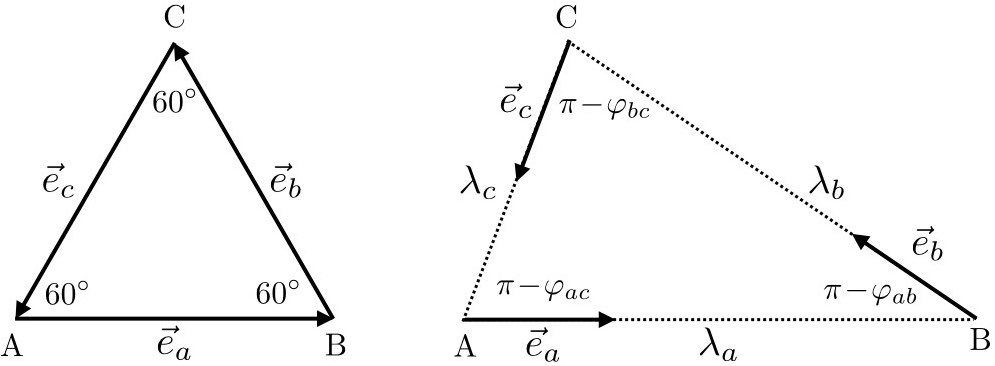
\includegraphics[width=4.5in]{vectors4elliptope.jpeg} 
   \caption{Coplanar peeling directions $(\vec{e}_a, \vec{e}_b, \vec{e}_c)$ resulting in triplets of correlation coeffients $(\chi_{ab}, \chi_{ac}, \chi_{bc})$ coordinatizing points on the surface of the elliptope in Figure \ref{elliptope}}
   \label{vectors4elliptope}
\end{figure}

As long as $(\vec{e}_a, \vec{e}_b, \vec{e}_c)$ are coplanar but no two of them are collinear, it will be possible for any triplet of values for 
\begin{equation}
\chi_{ab} = \cos{\varphi_{ab}} =  \vec{e}_a \! \cdot  \vec{e}_b, \quad \chi_{ac} =    \cos{\varphi_{ac}} =   \vec{e}_a \! \cdot \vec{e}_c, \quad \chi_{bc} =    \cos{\varphi_{bc}} \! = \!  \vec{e}_b \! \cdot \vec{e}_c
\label{chi's as inner prods of e's}
\end{equation}
on the surface of the elliptope to construct a triangle with sides of length $(\lambda_a, \lambda_b, \lambda_c)$ in the directions of the triplet of corresponding coplanar unit vectors $(\pm \vec{e}_a, \pm \vec{e}_b, \pm \vec{e}_c)$. If we need to flip one of the three unit vectors to form a triangle, we need to take minus the length of the corresponding side to satisfy Eq.\ (\ref{vecs add to 0}). If we can use $(\vec{e}_a, \vec{e}_b, \vec{e}_c)$ to form a triangle, the angles $(\varphi_{ab}, \varphi_{ab}, \varphi_{ab})$ will add up to $360\degree$. If we have to flip one of the unit vectors to do so, one of the angles will be the sum of the other two (cf.\ our discussion in Section \ref{1.5} of the angle inequalities in Eq.\ (\ref{angle inequalities})).  

This construction shows that by choosing the appropriate peeling directions in our quantum banana peeling and tasting experiment we can reach all points on the surface of the elliptope. In particular we can reach the point $(\chi_{ab}, \chi_{ac}, \chi_{bc}) = (-\sfrac12, -\sfrac12, -\sfrac12)$ at the center of the facet (ii)-(iii)-(iv) of the tetrahedron in Figure \ref{tetrahedron-angles} corresponding to the elliptope. For $v_a = v_b = v_c = 1$, Eq.\ (\ref{inf the 1}) reduces to 
\begin{equation}
\Big\langle \Big(  \frac{X_a}{\sigma_a} +  \frac{X_b}{\sigma_b} + \frac{X_c}{\sigma_c} \Big)^{\!2} \Big\rangle \ge 0.
\label{Tsirelson reprise 1}
\end{equation}
Eq.\ (\ref{inf the 4a}), with $\chi$'s substituted for $\overline{\chi}$'s (see Eq.\ (\ref{chi 4 bar-chi})), then turns into
\begin{equation}
3 + 2 \chi_{ab} + 2 \chi_{ac}  +  2 \chi_{bc} \ge 0.
\label{Tsirelson reprise 2}
\end{equation}
or
\begin{equation}
\chi_{ab} + \chi_{ac}  +  \chi_{bc} \ge -\sfrac32.
\label{Tsirelson reprise 3}
\end{equation}
The value $-\sfrac32$, which is just the Tsirelson bound we found in Section \ref{1.5} (see Eq.\ (\ref{Mermin Tsirelson bound on chis})), is reached at $(\chi_{ab}, \chi_{ac}, \chi_{bc}) = (-\sfrac12, -\sfrac12, -\sfrac12)$.

Note that the vector $\vec{\lambda} = (1, 1, 1)$ is an eigenvector with eigenvalue 0 of the anti-correlation matrix $\chi$ in Eq.\ (\ref{chi matrix}) with $(\chi_{ab}, \chi_{ac}, \chi_{bc}) = (-\sfrac12, -\sfrac12, -\sfrac12)$. If $\varphi_{ab} = \varphi_{ac} = \varphi_{bc} = 120\degree$, then
\begin{equation}
\chi = \begin{pmatrix}
1 & \chi_{ab} & \chi_{ac}  \\[.1cm]
\chi_{ab} & 1 & \chi_{bc} \\[.1cm]
\chi_{ac} & \chi_{bc} & 1
\end{pmatrix}
=
\begin{pmatrix}
1 & \cos{\varphi_{ab}} & \cos{\varphi_{ac}} \\[.1cm]
\cos{\varphi_{ab}} & 1 & \cos{\varphi_{bc}} \\[.1cm]
\cos{\varphi_{ac}} & \cos{\varphi_{bc}} & 1
\end{pmatrix}
=
\begin{pmatrix}
1 & -\sfrac12 & -\sfrac12 \\[.1cm]
-\sfrac12 & 1 & -\sfrac12 \\[.1cm]
 -\sfrac12 & -\sfrac12 & 1
\end{pmatrix}.
\label{chi 120 deg}
\end{equation}
Hence, for $\vec{\lambda} = (1, 1, 1)$, $\chi \, \vec{\lambda} = 0 \, \vec{\lambda}$:
\begin{equation}
\begin{pmatrix}
1 & \chi_{ab} & \chi_{ac}  \\[.1cm]
\chi_{ab} & 1 & \chi_{bc} \\[.1cm]
\chi_{ac} & \chi_{bc} & 1
\end{pmatrix} \!
\begin{pmatrix}
1 \\[.1cm]
1 \\[.1cm]
1
\end{pmatrix}
=
\begin{pmatrix}
0 \\[.1cm]
0 \\[.1cm]
0
\end{pmatrix}.
\label{eigenvector (111)}
\end{equation}

This is just one example of a general property. Let $(\chi_{ab}, \chi_{ac}, \chi_{bc})$ be the coordinates of any point on the surface of the elliptope that is not one of the four points the elliptope shares with the tetrahedron. Let $(\vec{e}_a, \vec{e}_b, \vec{e}_c)$ be a triplet of coplanar (but not collinear) unit vectors whose inner products give $(\chi_{ab}, \chi_{ac}, \chi_{bc})$ (see Eq.\ (\ref{chi's as inner prods of e's})). Let the coefficients $(\lambda_a, \lambda_b, \lambda_c)$, chosen in such a way that Eq.\ (\ref{vecs add to 0}) is satisfied, be the components of a vector $\vec{\lambda}$. This vector will be an eigenvector with eigenvalue 0 of the anti-correlation matrix $\chi$ for the values of $(\chi_{ab}, \chi_{ac}, \chi_{bc})$ in Eq.\ (\ref{chi's as inner prods of e's}). This is a direct consequence of  $\vec{\lambda}$ being an eigenvector with eigenvalue 0 of the matrix $L$ introduced in Section \ref{1.5} to write $\chi = L^\top L$ (see Eqs.\ (\ref{QM12})--(\ref{QM13})). That $L \, \vec{\lambda} = 0 \, \vec{\lambda}$, in turn, simply expresses the linear dependence of the three coplanar vectors $(\vec{e}_a, \vec{e}_b, \vec{e}_c)$. The columns of $L$ are just the components of $(\vec{e}_a, \vec{e}_b, \vec{e}_c)$. Using Eq.\ (\ref{comps of unit vectors e_abc}) for these components, one readily verifies that $L \, \vec{\lambda}$ vanishes:
\begin{eqnarray}
\begin{pmatrix}
a_x & b_x & c_x  \\
a_y & b_y & c_y  \\
a_z & b_z & c_x
\end{pmatrix} \!\!
\begin{pmatrix}
\lambda_a \\
\lambda_b \\
\lambda_c
\end{pmatrix}
& \! \! = \! \! &
\lambda_a \!
\begin{pmatrix}
a_x  \\
a_y \\
a_z
\end{pmatrix}
+
\lambda_b \!
\begin{pmatrix}
b_x  \\
b_y \\
b_z
\end{pmatrix}
+
\lambda_c \!
\begin{pmatrix}
c_x  \\
c_y \\
c_z
\end{pmatrix} \nonumber \\[-.2cm]
 & & \label{eigenvector of L} \\
 & \! \! = \! \! & \lambda_a \, \vec{e}_a + \lambda_b \, \vec{e}_b + \lambda_c \, \vec{e}_c = 0, \nonumber
\end{eqnarray}
where in the last step we used Eq.\ (\ref{vecs add to 0}). It follows that $\chi \vec{\lambda}$ also vanishes:
\begin{equation}
\begin{pmatrix}
\vec{e}_a \! \cdot   \vec{e}_a &  \vec{e}_a \! \cdot  \vec{e}_b  &   \vec{e}_a \! \cdot  \vec{e}_c  \\[.2cm]
\vec{e}_b \! \cdot  \vec{e}_a & \vec{e}_b \! \cdot  \vec{e}_b & \vec{e}_b \! \cdot  \vec{e}_c \\[.2cm]
\vec{e}_c \! \cdot  \vec{e}_a & \vec{e}_c \! \cdot  \vec{e}_b  & \vec{e}_c \! \cdot  \vec{e}_c
\end{pmatrix} \!
\begin{pmatrix}
\lambda_a \\[.2cm]
\lambda_b \\[.2cm]
\lambda_c
\end{pmatrix}
= \begin{pmatrix}
\, \vec{e}_a \! \cdot \! \big(\lambda_a \, \vec{e}_a + \lambda_b \, \vec{e}_b  + \lambda_c \, \vec{e}_c \big) \, \\[.2cm]
\, \vec{e}_b \! \cdot \! \big(\lambda_a \, \vec{e}_a + \lambda_b \, \vec{e}_b  + \lambda_c \, \vec{e}_c \big)  \, \\[.2cm]
\, \vec{e}_c \! \cdot \! \big(\lambda_a \, \vec{e}_a + \lambda_b \, \vec{e}_b  + \lambda_c \, \vec{e}_c \big)  \,
\end{pmatrix} =
\begin{pmatrix}
0 \\[.2cm]
0 \\[.2cm]
0
\end{pmatrix}.
\label{eigenvector lambda}
\end{equation}

One conclusion of the analysis in this subsection is that it is unsurprising that quantum mechanics does not allow any non-signaling correlations that violate the Tsirelson bound---or, more generally, any non-signaling correlations represented by points inside the non-signaling cube but outside the elliptope. This is not because of some elusive physical principle over and above non-signaling but simply because of the general constraint on (anti-)correlation coefficients in Eq.\ (\ref{inf the 5}). What \emph{is} surprising in light of this general constraint, is that the correlations allowed in our quantum banana peeling and tasting experiment get beyond the classical tetrahedron and fill out the entire elliptope. The taste of these bananas, after all, can only be $\pm \bbar/2$, regardless of what peeling is chosen, so it is impossible to find values for $X_a$, $X_b$ and $X_c$, representing the taste of a banana peeled $\hat{a}$, $\hat{b}$ and $\hat{c}$, respectively, such that $X_a + X_b + X_c = 0$. One would therefore expect the minimum value of the square of this sum to be $\bbar^2/4$ rather than 0. In that case, Eq.\ (\ref{Tsirelson reprise 1}) changes to
\begin{equation}
\Big\langle \Big(  \frac{X_a}{\sigma_a} +  \frac{X_b}{\sigma_b} + \frac{X_c}{\sigma_c} \Big)^{\!2} \Big\rangle \ge 1,
\label{CHSH reprise 1}
\end{equation} 
where we used that $\sigma_a = \sigma_b = \sigma_c = \bbar/2$ (see Eq.\ (\ref{standard deviations a and b})). Eq.\ (\ref{Tsirelson reprise 3}) would accordingly change to:
\begin{equation}
\chi_{ab} + \chi_{ac}  +  \chi_{bc} \ge - \sfrac32 + \sfrac12 = -1,
\label{CHSH reprise 2}
\end{equation}
which is just the CHSH-type inequality we found in Section \ref{1.4} (see Eq.\ (\ref{Mermin inequality CHSH-like})). As we saw above, the reason quantum mechanics is less restrictive is that it allows something no classical theory would allow, namely to assign a value to the sum of three variables without assigning a value to all three of them individually.

As illustrated by a simple example in \emph{Totally Random}, the speedup of a quantum computer comes from the ability to assign a truth value to a conjunction without having to assign a truth value to its conjuncts \citep[pp.\ 186--215]{Bub and Bub 2018}. Long before anybody was thinking about quantum computing, however, physicists had already run into a version of the conundrum encountered here and resolved by quantum mechanics. In their popular introductory textbook on quantum physics, \citet[p.\ 258]{Eisberg and Resnick 1985} highlight the peculiar behavior of angular momentum in quantum mechanics. That the wave function for a one-electron atom ``does not describe a state with a definite $x$ and $y$ component of orbital angular momentum,'' they note, ``is mysterious from the point of view of classical mechanics'' (and is equally mysterious for intrinsic or spin angular momentum). In quantum mechanics, they continue, this is required by the uncertainty principle. If the $z$-component has a definite value, the $x$- and $y$-components cannot have definite values.
 
\begin{figure}[h]
 \centering
   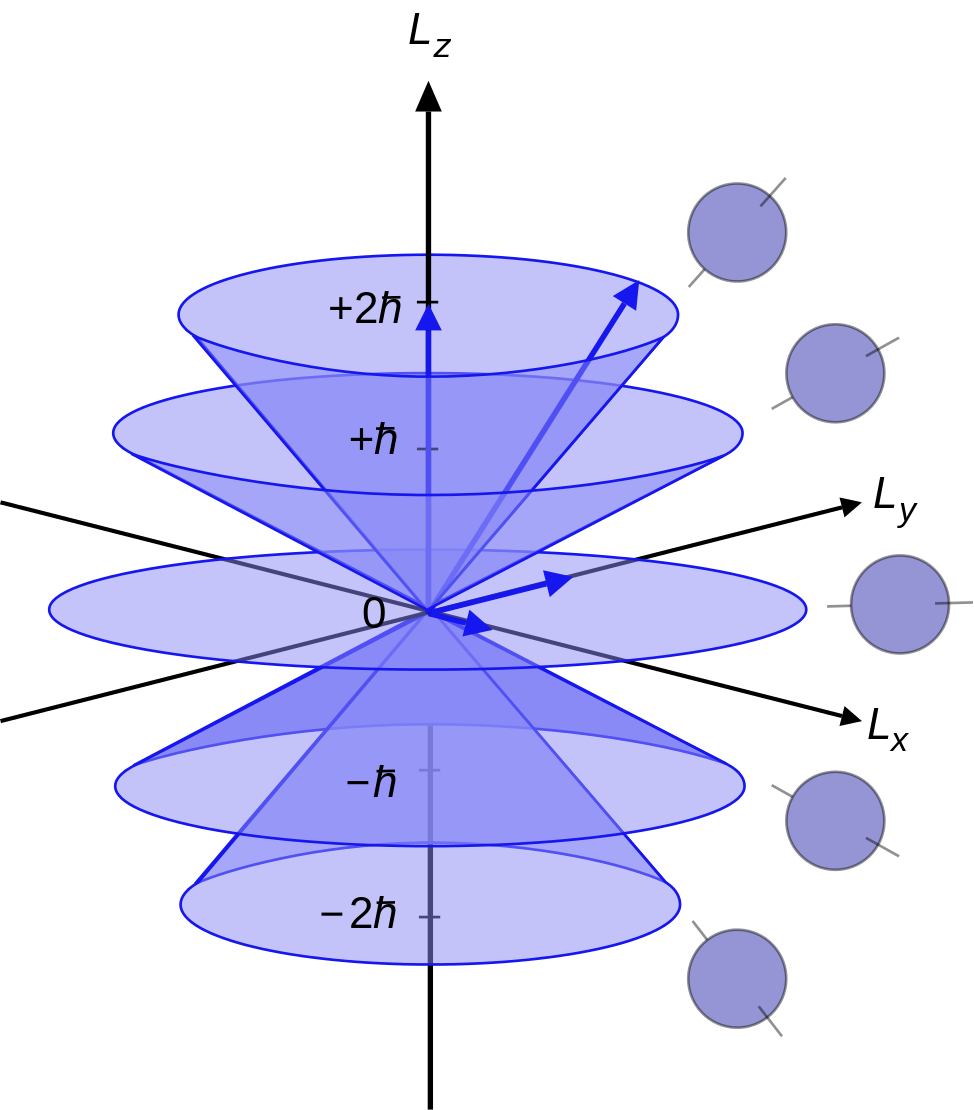
\includegraphics[width=2.6in]{Vector_model_of_orbital_angular_momentum.png} 
   \caption{Vector model of orbital angular momentum in the old quantum theory \citep[Wikimedia Commons; cf.][p.\ 258, Fig.\ 7-12]{Eisberg and Resnick 1985}. }
   \label{Vector_model_of_orbital_angular_momentum}
\end{figure}

This behavior of angular momentum,  \citet[pp.\ 258--259]{Eisberg and Resnick 1985} note in the next paragraph, ``can be conveniently represented by a \emph{vector model},'' i.e., the one shown in Figure \ref{Vector_model_of_orbital_angular_momentum}. In this model, the angular momentum vector precesses around the $z$ axis at a fixed angle determined by the value of its $z$-component. While the $z$-component remains fixed, the $x$- and $y$-components are constantly changing. This model, of course, still does not capture the true state of affairs in quantum mechanics where it is impossible to assign a definite value to all three component at any instant. The vector model is a left-over from the old quantum theory, where it was introduced to deal with problems posed by multiplet spectra and the anomalous Zeeman effect \citep[Sec.\ 1.3.6 and Ch.\ 7]{Duncan and Janssen 2019}.

The quantum-mechanical treatment of angular momentum not only solved these problems in spectroscopy, it also restored order in a completely different field. As John H.\ Van Vleck, the author of an authoritative book on the subject noted in the opening sentence of its preface: ``The new quantum mechanics  is perhaps most noted for its triumphs in the field of spectroscopy, but its less heralded successes in the theory of electric and magnetic susceptibilities must be regarded as one of its great achievements'' \citep[p.\ vii]{Van Vleck 1932}. Since we inserted this digression to preempt charges of parochialism against the information-theoretic interpretation of quantum mechanics we are championing (see Section \ref{0}), it is amusing to note that Van Vleck in the aftermath of the quantum revolution of the mid-1920s felt that he and his colleagues had been too focused on spectroscopy. In an article on the new quantum mechanics in a chemistry journal, he wryly noted that ``[t]he chemist is apt to conceive of the physicist as some one who is so entranced in spectral lines that he closes his eyes to other phenomena'' \citep[p.\ 493]{Van Vleck 1928}.\footnote{Both quotations are taken from \citet[p.\ 137]{Midwinter and Janssen 2013}. Van Vleck's solution to the problem of susceptibilities hinges on the correct quantum-mechanical treatment of angular momentum, in this case of diatomic molecules such as hydrogen chloride (ibid., p.\ 199). We will return to this episode in Section \ref{4.3a} as an example of a problem solved by the new kinematics of quantum mechanics.\label{Van Vleck}}

%SUBSECTION 2.6.3
\subsubsection{Further restrictions on the correlations generated by raffles meant to simulate the quantum correlations} \label{1.6.3}

We can find CHSH-type inequalities like the one in Eq.\ (\ref{CHSH reprise 2}) for raffles we will design in Section \ref{2.2} to simulate correlations found in measurements on pairs of entangled particles of spin $s  = 1, \sfrac32, 2, \sfrac52, \ldots$ in the singlet state. The spin in any direction (corresponding to the taste of a banana peeled in that peeling direction) will take on $2s \! + \! 1$ different values $m \hbar$, where $m = -s, -s+1, \ldots, s-1, s$ and $\hbar$ is Planck's constant divided by $2\pi$. We will analyze these quantum correlations in Section \ref{2.1}. 

\begin{figure}[h]
 \centering
   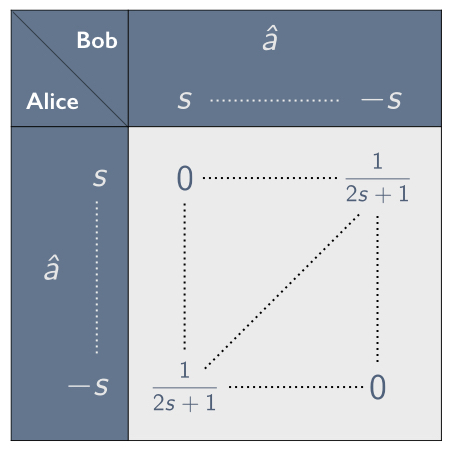
\includegraphics[width=2.5in]{diag-cell-sxs.jpeg} 
   \caption{Cell along the diagonal of a non-signaling correlation array with $2s+1$ outcomes per setting.}
   \label{diag-cell-sxs}
\end{figure}

Figure \ref{diag-cell-sxs} shows a cell along the diagonal of the correlation array for the quantum correlations for arbitrary spin $s$. It tells us that, when Alice and Bob use the same setting, all $2s \! + \! 1$ ways in which they can find opposite results (including $m = 0$ if $s$ is an integer) occur with equal probability. These quantum correlation arrays are non-signaling by virtue of having uniform marginals: in every row and every column of every cell, on or off the diagonal of the correlation array, the entries add up to $1/(2s \! + \! 1)$. 

In designing raffles for these higher-spin cases, we are immediately faced with a complication compared to the spin-$\frac12$ case (see Section \ref{2} for further discussion). Regardless of how many possible outcomes per setting there are, we can only put two outcomes per setting on any given ticket. This simple observation, unfortunately, has serious consequences for the design of our raffles. The reason we did not have to worry about this so far is that, for $s = \sfrac12$, there are only two possible outcomes per setting in the quantum experiment we are trying to simulate with our raffles. For $s > \sfrac12$, however, there are $2s+1$ possible outcomes per setting. Here is why this a problem. As we just saw, for any value of $s$, the quantum correlations are such that if Alice and Bob use the same setting, they are both expected to find all $2s+1$ possible outcomes in equal proportion. There is no way we can simulate this feature of the quantum correlations with single-ticket raffles as these tickets can at most have two of these $2s+1$ outcomes printed on them for each setting  (for integer values of $s$ it is possible that they have one and the same value, i.e., $0$, on both sides). In other words, for $s > \sfrac12$, the correlations we can produce with single-ticket raffles, while non-signaling by construction, do not give uniform marginals (see, e.g., Figure \ref{CA-3set3out-raffle-vi} in Section \ref{2.2}). To make sure that our raffles at least simulate the cells along the diagonal of the quantum correlation arrays correctly, we thus need to restrict ourselves to mixed raffles that do give uniform marginals. In Section \ref{2.2}, we will show how to construct those. All we need at this point is that any admissible raffle gives rise to a correlation array in which the cells along its diagonal have the form shown in Figure \ref{diag-cell-sxs}, which implies that they give uniform marginals.

Consider an arbitrary (single-ticket or mixed) raffle with tickets with opposite outcomes on the left and the right side for the three settings $\hat{a}$, $\hat{b}$ and $\hat{c}$ and with $2s \! + \! 1$ possible outcomes for each of these three settings. As in the case of two outcomes per setting considered so far, we can write:
\begin{equation}
\langle \left( X_a^A + X_b^A + X_c^A \right)^2 \rangle
= \sigma_a^2 + \sigma_b^2 + \sigma_c^2 - 2 \big( \langle X_a^A X_b^B \rangle + \langle X_a^A X_c^B \rangle + \langle X_b^A X_c^B \rangle \big)
\label{sum of X sq 4 any raffle}
\end{equation}
where, as before, we use $-X_a^A X_b^B$ as a proxy for $X_a^A X_b^A$, etc. 

The standard deviations are the square roots of variances computed for the cells along the diagonals of the relevant correlation arrays. Since these cells will all be of the form of the one in Figure \ref{diag-cell-sxs}, the three standard deviations in Eq.\ (\ref{sum of X sq 4 any raffle}) will have the same value $\sigma_s$, given by  
\begin{equation}
 \sigma_s^2 = \sigma_a^2 = \langle (X^A_a)^2 \rangle  \big|_{\mathrm{UM}}  = - \langle X^A_a X^B_a \rangle   \big|_{\mathrm{UM}}, 
\label{SD for adm raffle 1}
\end{equation}
where $ \big|_{\mathrm{UM}}$ indicates that the (co-)variance be evaluated for a raffle giving uniform marginals. Inspection of Figure \ref{diag-cell-sxs} and the well-known sum-of-squares formula gives
\begin{equation}
\sigma_s^2 = - \sum_{m=-s}^s \! \frac{(m \, \hbar) (-m \, \hbar)}{2s+1} = \frac{\hbar^2}{2s+1} \sum_{m=-s}^s \!\! m^2 =  \frac13 s(s+1) \, \hbar^2.
\label{SD for adm raffle 2}
\end{equation}

For raffles giving uniform marginals, we have
\begin{equation}
\chi_{ab}   \big|_{\mathrm{UM}} = \left. - \left( \frac{\langle X_a^A X_b^B \rangle}{\sigma_a \sigma_b} \right) \right|_{\mathrm{UM}} = - \frac{1}{\sigma_s^2} \langle X_a^A X_b^B \rangle   \big|_{\mathrm{UM}}.\label{chi and covariance adm raffle}
\end{equation}
Similar expressions obtain for $\chi_{ac}$ and $\chi_{bc}$. For such raffles, Eq.\ (\ref{sum of X sq 4 any raffle}) can be rewritten as
\begin{equation}
\langle \left( X_a^A + X_b^A + X_c^A \right)^2 \rangle  \big|_{\mathrm{UM}}
= \sigma_s^2 \left( 3 + 2 \! \left. \big( \chi_{ab} + \chi_{ac} + \chi_{bc} \big) \right|_{\mathrm{UM}} \right).
\label{sum of X sq 4 UM raffle}
\end{equation}

For any half-integer value of $s$, $|X_a^A + X_b^A + X_c^A|$ cannot be made smaller than $\hbar/2$, hence
\begin{equation}
\langle \left( X_a^A + X_b^A + X_c^A \right)^{\!2} \rangle \ge \frac{\hbar^2}{4} \quad {\mathrm{for \; half}}\mbox{-}{\mathrm{integer \;}} s.
\label{De Finetti half integer s}
\end{equation}
For any integer value of $s$, $X_a + X_b + X_c$ can be made to vanish, hence
\begin{equation}
\langle \left( X_a^A + X_b^A + X_c^A \right)^{\!2} \rangle \ge 0 \quad {\mathrm{for \; integer \;}} s.
\label{De Finetti integer s}
\end{equation} 
Restricting ourselves to raffles giving uniform marginals, in which case we can use Eq.\ (\ref{sum of X sq 4 UM raffle}), we thus find the following CHSH-type lower bounds on the sum of the anti-correlation coefficients in the Mermin setup:
\begin{equation}
\big( \chi_{ab} + \chi_{ac} + \chi_{bc} \big)  \big|_{\mathrm{UM}} \ge \frac{\hbar^2}{8\sigma_s^2} - \frac32 \quad {\mathrm{for \; half}}\mbox{-}{\mathrm{integer \;}} s,
\label{Mermin CHSH half-integer spin}
\end{equation}
\begin{equation}
\big( \chi_{ab} + \chi_{ac} + \chi_{bc} \big)  \big|_{\mathrm{UM}}  \ge - \frac32 \quad {\mathrm{for \; integer \;}} s.
\label{Mermin CHSH integer spin}
\end{equation}
For $s=\sfrac12$, $\sigma_s^2 = \hbar^2/4$ and Eq.\ (\ref{Mermin CHSH half-integer spin}) reduces to Eq.\ (\ref{CHSH reprise 2}), the CHSH-like inequality for this setup (since all raffles for the spin-$\frac12$ case give uniform marginals, the restriction $\big|_{\mathrm{UM}}$ can be dropped).

Eq.\ (\ref{Mermin CHSH integer spin}) tells us that, for integer values of $s$, we can (at least in principle) always reach the Tsirelson bound for a Mermin setup with $2s+1$ outcomes per setting (in Section \ref{2.2} we will design raffles that do indeed reach this bound). Eq.\ (\ref{Mermin CHSH half-integer spin}) tells us that, for half-integer values of $s$, this is true only in the limit that $s$ goes to infinity, in which case the number of outcomes $2s+1$ and the standard deviation $\sigma_s$ also go to infinity. 

As we will show in detail for the $s=1$ case in Section \ref{2.2}, even though we \emph{can} reach the Tsirelson bound on the sum of (anti-)correlation coefficients with our raffles, these raffles still \emph{cannot} reproduce all individual entries in the correlation arrays for the quantum correlations they are supposed to simulate (see Eq.\ (\ref{off diag cell quantum v raffle})). The reason for this will also become clear in Section \ref{2}. In Section \ref{2.1}, we will show that, regardless of the spin $s$ of the two particles involved, the probabilities in any given cell in these quantum correlation arrays can still be parametrized by the angle between measuring directions. In Section \ref{2.2}, we will see that in our raffles this is true only for the simple case $s = \sfrac12$ of two outcomes per setting that we have been considering so far. Even in the case of $s=1$, we already need two parameters to specify the entries in any off-diagonal cell in our correlation arrays (see Figure \ref{symmetry-spin-1-32}). We will give a simple example of measurements one could in principle do on two spin-1 particles entangled in the singlet state where quantum mechanics predicts results that cannot be accounted for in any local hidden-variable theory \emph{even though these results do not violate the relevant Bell inequality}.

%SUBSECTION 2.6.4
\subsubsection{The geometry of correlations: from Pearson and Yule to Fisher and de Finetti} \label{1.6.4}

In this subsection, we indicate how \citet{Yule 1896} found the general constraint on correlation coefficients in Eq.\ (\ref{inf the 5}) in the context of regression theory (i.e., finding the straight lines best approximating correlations between variables) and how \citet{Fisher 1915,Fisher 1924} and \citet{De Finetti 1937} recovered the result Yule found algebraically by treating random variables as vectors and correlations in terms of angles between those vectors. The importance of this geometric approach was emphasized by \citet{Pearson 1916}:
\begin{quote}
It is greatly to be desired that the ``trigonometry'' of higher dimensioned plane space should be fully worked out, for all our relations between multiple correlation and partial correlation coefficients of $n$ variates are properties of the ``angles,'' ``edges'' and ``perpen\-diculars'' of sphero-polyhedra in multiple space. It would be a fine task for an adequately equipped pure mathematician to write a treatise on ``spherical polyhedrometry''; he need not fear that his results would be without practical application for they embrace the whole range of problems from anatomy to medicine and from medicine to sociology and ultimately to the doctrine of evolution \citep[p.\ 237]{Pearson 1916}.\footnote{Linear algebra has proven to be much more convenient than spherical geometry for dealing with the relevant problems in statistics. As \citet[p.\ 73]{Aldrich 1998} notes, ``[t]he treatise on the trigonometry of correlations \ldots\ never materialized. [Kendall, 1961] is a partial offering but it appeared just as a new approach was taking off. This drew on the Hilbert space theory developed in the early part of the century and assembled by [Stone 1932].''}
\end{quote}
Rather than discussing the geometry of correlations in the abstract, we use the concrete example of three balanced random variables $(X_a, X_b, X_c)$ illustrated in Figure \ref{3M-balance}. 

\begin{figure}[h!]
 \centering
   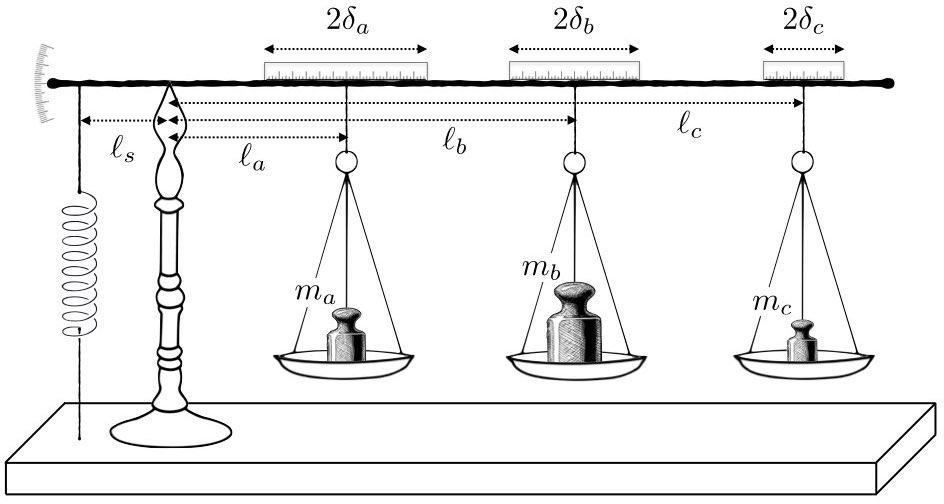
\includegraphics[width=5in]{3M-balance.jpeg} 
   \caption{3$m$ balance: an elementary example of a correlation between three random variables $(X_a, X_b, X_c) \equiv (\Delta \ell_a, \Delta \ell_b, \Delta \ell_c)$ (with $| \Delta \ell_a | \le \delta_a$, $| \Delta \ell_b | \le \delta_b$ and $| \Delta \ell_c | \le \delta_c$).}
   %The values for the displacements $(\Delta \ell_a, \Delta \ell_b, \Delta \ell_c)$ from the points $(\ell_a, \ell_b,  \ell_c)$ are subject to the constraint that the torque coming from the three scale pans on the right (with masses $m_a$, $m_b$ and $m_c$) in them exactly cancels the opposing torque coming from the spring on the left, so that the beam remains horizontal as it is for $(\Delta \ell_a, \Delta \ell_b, \Delta \ell_c) = (0, 0, 0)$.
   \label{3M-balance}
\end{figure} 

This figure shows a device we will call a \emph{3m balance}, so named for the three masses $m_a$, $m_b$ and $m_c$ in the scale pans hanging from its beam. In the configuration shown in the figure, the three pans are at distances $\ell_a$, $\ell_b$ and $\ell_c$ from the beam's pivot point. In this configuration, the torque coming from the three pans on the right exactly cancels the torque coming from the spring on the left:   
\begin{equation}
F_s \ell_s = g \big( m_a \, \ell_a + m_b \, \ell_b + m_c \, \ell_c \big).
\label{torques}
\end{equation}
Here $F_s$ is the force exerted by the spring, $\ell_s$ its distance to the pivot point and $g$ the acceleration of gravity. Now imagine we take these three pans off the beam and put them back on (with the same masses as before) such that (a) the system is once again perfectly balanced (i.e., the beam is horizontal) and (b) the pans with $m_a$, $m_b$ and $m_c$ are somewhere in the intervals  $\ell_a \pm \delta_a$, $\ell_b \pm \delta_b$ and $\ell_c \pm \delta_c$, respectively. Suppose we end up putting the pans at the displaced positions
\begin{equation}
\ell_a + \Delta \ell_a, \quad \ell_b + \Delta \ell_b, \quad \ell_c + \Delta \ell_c,
\end{equation}
where $| \Delta \ell_a | \le \delta_a$, $| \Delta \ell_b | \le \delta_b$ and $| \Delta \ell_c | \le \delta_c$. The displacements $(\Delta \ell_a, \Delta \ell_b, \Delta \ell_c)$ that characterize this new perfectly balanced configuration of the system will satisfy the linear equation
\begin{equation}
m_a \, \Delta \ell_a + m_b \, \Delta\ell_b + m_c \, \Delta \ell_c  = 0.
\label{lin rel delta l}
\end{equation}
Suppose we repeat this many times.
%experiment of taking the three pans off the beam and putting them back on many times. 
The triplets of displacements $(\Delta \ell_a, \Delta \ell_b, \Delta \ell_c)$ found in consecutive runs of this experiment, all satisfying Eq.\ (\ref{lin rel delta l}), can then be treated as triplets of values for the three random variables
\begin{equation}
(X_a, X_b, X_c) \equiv (\Delta \ell_a, \Delta \ell_b, \Delta \ell_c).
\label{X = delta l}
\end{equation}
Since we are equally likely to find $\Delta \ell_a$ as $-\Delta \ell_a$, $\Delta \ell_b$ as $-\Delta \ell_b$ and $\Delta \ell_c$ as $-\Delta \ell_c$, these variables are 
balanced (see the definition numbered (\ref{def balanced}) in Section \ref{1.3}).\footnote{Since $X_a$ is balanced, its expectation value is zero and its variance is given by
\begin{equation*}
\langle (X_a - \langle X_a \rangle)^2 \rangle = \langle X_a^2 \rangle = \frac{1}{2\delta_a} \int_{-\delta_a}^{\delta_a} \!\! X_a^2 \, dX_a =  \frac{1}{6\delta_a} X_a^3 \Big|_{-\delta_a}^{\delta_a} = \frac{\delta_a^2}{3}.
\label{variance 3M variable} 
\end{equation*}
The corresponding standard deviation is: $\sigma_a \! = \! \sqrt{\langle X_a^2 \rangle} \! = \! \delta_a/\sqrt{3}$. Similarly, $\sigma_b  \! = \!  \delta_b/\sqrt{3}$ and $\sigma_c  \! = \!   \delta_c/\sqrt{3}$.\label{3M balance SDs}} They are correlated: if we vary the position of one of the masses, we need to vary the position of at least one of the other two to satisfy Eq.\ (\ref{lin rel delta l}). This is expressed by the linear relation
\begin{equation}
m_a \, X_a + m_b \, X_b + m_c \, X_c  = 0
\label{lin rel X_abc}
\end{equation}
between the three variables, which is just Eq.\ (\ref{lin rel delta l}) with $\Delta \ell$ replaced by $X$.

Note that in this simple example there is no problem obtaining values for all three variables in every run. In our quantum banana peeling and tasting experiment, we could only ascertain the values (tastes) for two of the three variables (peelings). The experiment with our 3$m$ balance, however, does share several features with both our quantum banana experiment and the raffles meant to simulate them. As with any three balanced random variables the allowed values for the corresponding three correlation coefficients $(\chi_{ab}, \chi_{ac}, \chi_{bc})$ are bound by the elliptope. The correlation will be represented by a point on the surface of the elliptope if some linear combination of the three variables (or, in the quantum case, \emph{the operator representing} the three variables) gives zero. Eq.\ (\ref{lin rel X_abc}) gives this linear combination in the case of the 3$m$ balance. This relation will hold as long as we can ignore errors in our measurement of the displacements $(\Delta \ell_a, \Delta \ell_b, \Delta \ell_c)$ and as long as there are no other masses pulling on the balance's beam. We can represent both of these complicating factors by an additional pan containing some unknown mass pulling on the beam at some unknown location. In that case, the right-hand side of Eq.\ (\ref{lin rel X_abc}) is no longer zero. That, in turn, means that the correlation between these three variables will be represented by a point inside the elliptope rather than on its surface.\footnote{This provides a simple way to understand a comment by Richard Holt, the second H in CHSH, in an interview in 2001 about finding a result in an early test of the CHSH inequality that did not agree with the quantum-mechanical prediction: ``whenever you're looking for a stronger correlation, any kind of systematic error you can imagine typically weakens it and moves it toward the hidden-variable range'' \citep[p.\ 286]{Gilder 2008}.} 

If we set $m_a = m_b = m_ c =m$ and $\delta_a = \delta_b = \delta_c = \delta$  and only allow the values $\pm \delta/2$ for the variables $X_a$, $X_b$ and $X_c$, their sum can no longer be made to vanish. To balance the beam in this case we need to put our thumb on the scale. This too can be represented by an additional pan on the beam. This pan must provide a torque of $mg\delta/2$ to compensate for the smallest torque possible coming from the other three pans combined. The quantity $\left(X_a + X_b + X_c \right)^2$ can never be less than $\delta^2/4$ in this case and we can no longer reach the point $(\chi_{ab}, \chi_{ac}, \chi_{bc}) = 
%(-\delta/2, -\delta/2, -\delta/2)$ 
(-\sfrac12, -\sfrac12, -\sfrac12)$ corresponding to the Tsirelson bound in our quantum banana experiment. Instead we find ourselves right back where we were when we tried to design a raffle to simulate the correlations found in the quantum banana peeling and tasting experiment (cf.\ Eqs.\ (\ref{Tsirelson reprise 1})--(\ref{CHSH reprise 2}) above). 

In our discussion of the 3$m$ balance so far, we have tacitly assumed that we know the masses in the three pans and thus the coefficients in the linear relation between $X_a$, $X_b$ and $X_c$ in Eq.\ (\ref{lin rel X_abc}) that tells us how these three variables are correlated. Typically we will not know those coefficients. Pearson, Yule and Fisher were especially interested in biological variables. These will seldom satisfy a simple linear relation such as the one Eq.\ (\ref{lin rel X_abc}). Suppose, however, that we have reason to believe that three balanced random variables do satisfy a linear relation of this form, with unknown coefficients and a non-zero right-hand side. In terms of our 3$m$ balance this corresponds to the situation in which we do not know the masses in the three pans and cannot rule out that there is a fourth pan somewhere on the beam with another unknown mass. We run the same experiment as before in which we repeatedly put the three pans on the beam somewhere within the allowed intervals always making sure the beam is balanced. Say, we repeat this experiment $n \gg 1$ times. That gives us $n$ triplets of values for $(X_a, X_b, X_c)$. We now plot, say, $X_b$ against $X_a$. Eq.\ (\ref{lin rel X_abc}) with the right-hand side changed from 0 to $U$ (for ``unknown torque'') tells us that
\begin{equation}
X_b  = - \left(\frac{m_a }{m_b} \right) X_a - \left( \frac{m_c}{m_b} \right) X_c \, + \; \frac{U}{m_b}.   
\end{equation}
On the assumption that $U$ does not change much over the course of the $n$ runs and given that for any value of $X_c$ we find we are as likely to find its opposite, the slope of the straight line in our plot of $X_b$ against $X_a$ that best fits the data is a good estimate of the ratio $m_a/m_b$. Plotting $X_c$ against $X_a$, we likewise obtain a good estimate of the ratio $m_a/m_c$. If we are told the value of $m_a$, our experiment thus gives us good estimates of $m_b$ and $m_c$. This is a simple example of regression analysis. It is in this context that Yule studied correlations. Instead of following Yule's algebraic approach, however, we switch to the geometric approaches of Fisher and de Finetti.

For our use of \citet{Fisher 1915, Fisher 1924}, we rely on the paper mentioned at the beginning of this section by \citet[sec.\ 10, pp.\ 72--74; see also Kendall, 1961, pp.\ 55--57]{Aldrich 1998}. Think of the values for the random variables $X_a$, $X_b$ and $X_c$ found in runs $1, 2, \ldots n$ ($n \gg 1$) of our experiment with the 3$m$ balance as the components of the $n$-dimensional vectors
\begin{equation}
\vec{X}^{(n)}_a \equiv \big( X_a^1, \dots X_a^n \big), \; \vec{X}^{(n)}_b \equiv \big( X_b^1, \dots X_b^n \big), \; 
\vec{X}^{(n)}_c \equiv \big( X_c^1, \dots X_c^n \big).
\label{sample vectors}
\end{equation}
We will call such vectors \emph{representative sample vectors}. A sample vector is representative if its components form a balanced sample, i.e., if (a) $\pm X_a, \pm X_b, \pm X_c$ occur with equal frequency and (b) $\sum_{k=1}^n X_a^k = \sum_{k=1}^n X_b^k = \sum_{k=1}^n X_c^k = 0$.\footnote{Here is how we construct a representative sample vector of dimension $n = 2m$ if we only perform a relatively small number $m$ runs of the experiment. For the first $m$ components of the sample vectors $(\vec{X}^{(n)}_a, \vec{X}^{(n)}_b, \vec{X}^{(n)}_c)$, we use the values for $X_a$, $X_b$ and $X_c$ found in these runs; for the last $m$ components, we use \emph{minus} these values. This construction guarantees that the samples from which the sample vectors are constructed are balanced.}

The standard dot product of $\vec{X}^{(n)}_a$ with itself gives $n$ times the variance of $X_a$:
\begin{equation}
\vec{X}^{(n)}_a \! \cdot \! \vec{X}^{(n)}_a = \sum_{k=1}^n \big(X_a^k)^2 = n \langle X_a^2 \rangle = n \, \sigma_a^2,
\label{dot product aa}
\end{equation}
where $\sigma_a$ is the standard deviation. Similar results hold for the dot products of $\vec{X}^{(n)}_b$ and $\vec{X}^{(n)}_c$ with themselves. Hence 
\begin{equation}
\| \vec{X}^{(n)}_a \| = \sqrt{n} \, \sigma_a, \quad \| \vec{X}^{(n)}_b \| = \sqrt{n} \, \sigma_b, \quad \| \vec{X}^{(n)}_c \| = \sqrt{n} \, \sigma_c.
\label{dot products aa bb cc}
\end{equation}
The dot product of $\vec{X}^{(n)}_a$ and $\vec{X}^{(n)}_b$ gives $n$ times the covariance of $X_a$ and $X_b$:
\begin{equation}
\vec{X}^{(n)}_a \! \cdot \! \vec{X}^{(n)}_b = \sum_{k=1}^n  X_a^k  X_b^k = n \langle X_a X_b \rangle.
\label{dot product ab}
\end{equation}
We can use these dot products to define angles between sample vectors. The cosines of these angles are just the Pearson correlation coefficients in Eq.\ (\ref{corr coeff gen})). We verify this for the cosine of the angle $\vartheta_{ab}$ between $\vec{X}^{(n)}_a$ and $\vec{X}^{(n)}_b$:
\begin{equation}
\cos{\vartheta_{ab}} = \frac{\vec{X}^{(n)}_a \! \cdot \! \vec{X}^{(n)}_b}{\| \vec{X}^{(n)}_a \| \| \vec{X}^{(n)}_b \|} = \frac{n  \langle X_a X_b \rangle}{\sqrt{n} \, \sigma_a \, \sqrt{n} \, \sigma_b} =
 \frac{\langle X_a X_b \rangle}{ \sigma_a \sigma_b} = \overline{\chi}_{ab}.
\label{sample vectors a b angle}
\end{equation}

\begin{figure}[h!]
 \centering
   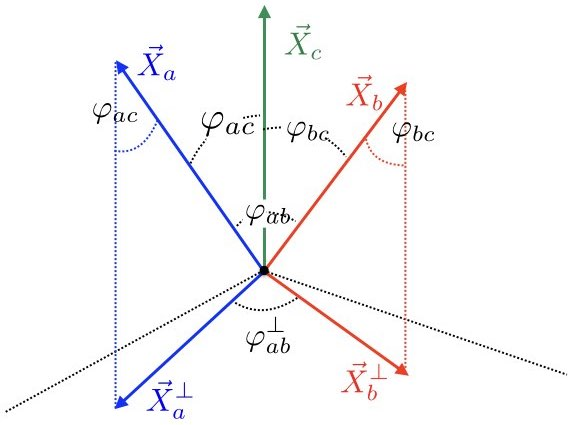
\includegraphics[width=4in]{vectors4yule.jpeg} 
   \caption{Vectors representing balanced samples of triplets of values of the random variables $(X_a, X_b, X_c)$.}
   \label{vectors4yule}
\end{figure}

Suppressing the superscripts $(n)$, we now decompose the sample vectors $\vec{X}_a$ and $\vec{X}_b$ into components parallel and perpendicular to the sample vector $\vec{X}_c$:
\begin{equation}
\vec{X}_a = \vec{X}_a^\parallel + \vec{X}_a^\perp, \quad \vec{X}_b = \vec{X}_b^\parallel + \vec{X}_b^\perp
\label{split per par}
\end{equation}
This decomposition is illustrated in Figure \ref{vectors4yule}. The parallel components can be seen as measures of the correlation between the random variables $X_a$ and $X_c$ and the correlation between $X_b$ and $X_c$; the perpendicular components as measures of the so-called partial or residual correlation between $X_a$ and $X_b$ \citep[p.\ 73]{Aldrich 1998}.\footnote{As we saw in Section \ref{1.5}, the tastes two bananas, one peeled $\hat{a}$ by Alice, the other peeled $\hat{b}$ by Bob, are completely \emph{uncorrelated} if the peeling directions $\vec{e}_a$ and $\vec{e}_b$ are orthogonal. It follows that the geometry of these sample vectors differs from the geometry of state vectors in Hilbert space in quantum mechanics. We will return to this point in the context of our discussion of \citet{De Finetti 1937} below.\label{orthogonal preview}} As Fisher put it (translated into our notation): 
\begin{quote}
[T]he correlation between [$X_a$] and [$X_b$] \ldots\ will be the cosine of the angle between  [$\vec{X}_a$] and [$\vec{X}_b$] \ldots\
[T]he partial correlation between [$X_a$] and [$X_b$] is the cosine of the angle between the projections of [$\vec{X}_a$] and [$\vec{X}_b$] upon the region perpendicular to [$\vec{X}_c$]
\citep[pp.\ 329--330]{Fisher 1924}.
\end{quote}
The lengths of the parallel and perpendicular components of $\vec{X}_a$ and $\vec{X}_b$  are
\begin{equation}
\begin{array}{c}
 \| \vec{X}_a^\parallel \| \! = \!  \|  \vec{X}_a  \| \cos{\vartheta_{ac}} \! = \!  \sqrt{n} \, \sigma_a \cos{\vartheta_{ac}}, \quad
\| \vec{X}_a^\perp \| \! = \!  \|  \vec{X}_a  \| \sin{\vartheta_{ac}} \! = \!   \sqrt{n} \, \sigma_a \sin{\vartheta_{ac}},    \\[.4cm]
\| \vec{X}_b^\parallel \| \! = \!  \|  \vec{X}_b  \| \cos{\vartheta_{bc}} \! = \!   \sqrt{n} \, \sigma_b \cos{\vartheta_{bc}}, \quad
\| \vec{X}_b^\perp \| \! = \!  \|  \vec{X}_b  \| \sin{\vartheta_{bc}} \! = \!  \sqrt{n} \, \sigma_b \sin{\vartheta_{bc}}, 
\end{array}
\label{lengths per par}
\end{equation}
where we used Eq.\ (\ref{dot products aa bb cc}) for $ \|  \vec{X}_a  \|$ and $ \|  \vec{X}_b  \|$. 

We can rewrite the dot product in Eq.\ (\ref{sample vectors a b angle}) as
\begin{equation}
\cos{\vartheta_{ab}} = \frac{\big( \vec{X}_a^\parallel + \vec{X}_a^\perp \big) \! \cdot \! \big(  \vec{X}_b^\parallel + \vec{X}_b^\perp \big)}{n \sigma_a \sigma_b}
= \frac{\vec{X}_a^\parallel \! \cdot \! \vec{X}_b^\parallel + \vec{X}_a^\perp \! \cdot \! \vec{X}_b^\perp}{n \sigma_a \sigma_b}.
\label{cos theta ab}
\end{equation}
With the help of Eq.\ (\ref{lengths per par}), the parallel components of $\vec{X}_a$ and $\vec{X}_b$ can be written as
\begin{equation}
\begin{array}{c}
\vec{X}_a^\parallel = \| \vec{X}_a \| \cos{\vartheta_{ac}} \displaystyle{\frac{\vec{X}_c}{\| \vec{X}_c \|}} = \displaystyle{\frac{\sigma_a}{\sigma_c}} \cos{\vartheta_{ac}} \, \vec{X}_c, 
\\[.5cm]
\vec{X}_b^\parallel = \| \vec{X}_b \| \cos{\vartheta_{bc}} \displaystyle{\frac{\vec{X}_c}{\| \vec{X}_c \|}} = \displaystyle{\frac{\sigma_b}{\sigma_c}} \cos{\vartheta_{bc}} \, \vec{X}_c.
\end{array}
\label{ab par vecs and vec c} 
\end{equation}
Using these expressions along with $\vec{X}_c \! \cdot \! \vec{X}_c = \| \vec{X}_c \|^2 = n \, \sigma_c^2$, we can write the dot product of the parallel components of $\vec{X}_a$ and $\vec{X}_b$ as
\begin{equation}
\vec{X}_a^\parallel \! \cdot \! \vec{X}_b^\parallel = n \, \sigma_a \sigma_b \cos{\vartheta_{ac}} \cos{\vartheta_{bc}}.
\label{dot par comps}
\end{equation}
The dot product of the perpendicular components can be written as
\begin{equation}
\vec{X}_a^\perp \! \cdot \! \vec{X}_b^\perp = \| \vec{X}_a^\perp \| \| \vec{X}_b^\perp \|   \cos{\vartheta_{ab}^\perp} =
n \, \sigma_a \sigma_b \sin{\vartheta_{ac}} \sin{\vartheta_{bc}} \cos{\vartheta_{ab}^\perp},
\label{dot perp comps}
\end{equation}
where, once again, we used Eq.\ (\ref{lengths per par}). Inserting Eqs.\ (\ref{dot par comps})--(\ref{dot perp comps}) into Eq.\ (\ref{cos theta ab}), we arrive at
\begin{equation}
\cos{\vartheta_{ab}} = \cos{\vartheta_{ac}} \cos{\vartheta_{bc}} + \sin{\vartheta_{ac}} \sin{\vartheta_{bc}} \cos{\vartheta_{ab}^\perp}.
\label{cos theta ab 2}
\end{equation}
Solving for $\cos{\vartheta_{ab}^\perp}$, we find that\footnote{If all vectors in Figure \ref{vectors4yule} are turned into unit vectors so that there tips all lie on a unit sphere, one easily recognizes that Eq.\ (\ref{cos theta ab perp}) is nothing but the spherical law of cosines. This illustrates the observation by Pearson quoted at the beginning of this subsection. The relation between the ``full'' and the partial correlation between $X_a$ and $X_b$ is thus fairly trivial. Borrowing a comment by \citet[p.\ 73]{Aldrich 1998} on a closely related aspect of Fisher's analysis, we can say that Fisher's derivation of this formula for the partial correlation amounts to ``something of a self-annihilating insight.''}
\begin{equation}
\cos{\vartheta_{ab}^\perp} = \frac{\cos{\vartheta_{ab}} - \cos{\vartheta_{ac}} \cos{\vartheta_{bc}}}{\sin{\vartheta_{ac}} \sin{\vartheta_{bc}}}. 
\label{cos theta ab perp}
\end{equation}
If $\overline{\chi}$'s are substituted for cosines of $\vartheta$'s and expressions of the form $\sqrt{\big( 1 - \overline{\chi}^2 \big)}$ for sines of $\vartheta$, this turns into:
\begin{equation}
\cos{\vartheta_{ab}^\perp} = \frac{\overline{\chi}_{ab} - \overline{\chi}_{ac} \overline{\chi}_{bc}}{\sqrt{\big( 1 - \overline{\chi}_{ac}^2 \big)} \sqrt{\big( 1 - \overline{\chi}_{bc}^2 \big)}}. 
\label{elliptope Yule 1}
\end{equation}
The quantity on the right-hand side can be found in \citet[p.\ 485]{Yule 1896}, who denotes it as $\rho_{12}$ and calls it the ``net coefficient of correlation between $x_1$ and $x_2$'' ($X_a$ and $X_b$ in our notation; Yule's $x_3$, likewise, is $X_c$ in our notation). Squaring both sides of Eq.\ (\ref{elliptope Yule 1}) we find:
\begin{equation}
\cos^2{\! \vartheta_{ab}^\perp} = \frac{ \big( \overline{\chi}_{ab} - \overline{\chi}_{ac} \overline{\chi}_{bc} \big)^2}{\big(1 - \overline{\chi}_{ac}^2 \big) \big( 1 - \overline{\chi}_{bc}^2 \big)}.
\label{elliptope Yule 2}
\end{equation}
Since $\cos^2{\! \vartheta_{ab}^\perp} \le 1$, we have the inequality \citep[p.\ 486]{Yule 1896}
\begin{equation}
  \big(\overline{\chi}_{ab} - \overline{\chi}_{ac} \overline{\chi}_{bc} \big)^2 \; \le \; \big( 1 - \overline{\chi}_{ac}^2 \big) \big( 1 - \overline{\chi}_{bc}^2 \big);
  \label{lastminute}
\end{equation}
or, expanding both sides,  
\begin{equation}
\overline{\chi}_{ab}^2 - 2 \overline{\chi}_{ab} \overline{\chi}_{ac} \overline{\chi}_{bc} + \overline{\chi}_{ac}^2 \overline{\chi}_{bc}^2
\; \le \; 1 - \overline{\chi}_{ac}^2 - \overline{\chi}_{bc}^2 + \overline{\chi}_{ac}^2 \overline{\chi}_{bc}^2.
\label{elliptope deja vu}
\end{equation}
The terms $\overline{\chi}_{ac}^2 \overline{\chi}_{bc}^2$ before and after the `$\le$' cancel and we see that this inequality is equivalent to the one in Eq.\ (\ref{inf the 5}) that defines the elliptope.

The construction above with sample vectors is problematic as probabilities only coincide with relative frequencies in the $n\to\infty$ limit. 
%{\michael There should probably be more elaboration about why it's objectionable.}
To remedy this, we consider the random variables themselves as vectors. This is actually a common approach in modern probability theory \citep[see, e.g.,][]{Fristedt and Gray 1997}. An early instance of it can be found in a paper of \citet{De Finetti 1937}.\footnote{We used the translation by Luca Barone and Peter Laurence, who also co-authored a commentary on the paper \citep{Laurence 2008}.}

De Finetti begins his geometric interpretation by observing that ``since we can consider linear combinations of random variables, we can interpret them as vectors in an `abstract space'\,'' \citep[p.\ 5]{De Finetti 1937}.\footnote{Unless noted otherwise, page references in the remainder of this section are to \citet{De Finetti 1937} } That is to say, linear combinations of random variables are also random variables and so form a vector space. Standard deviations can be interpreted as the norm of vectors in this space (cf.\ Eqs.\ (\ref{dot product aa})--(\ref{dot products aa bb cc}) for Fisher's sample vectors), 
\begin{equation}
\| X\| \equiv \sqrt{\langle X^2 \rangle}.
\end{equation}
%which we may recognize as the $L^2$-norm with respect to the probability measure $P$. 
The distance (or metric) between two random variables $X$ and $Y$ can then be defined as:\footnote{One subtlety of this definition is that $d(X,Y)=0$ when $X$ and $Y$ differ by a constant random variable (i.e., a random variable guaranteed to have the same value every time it is measured). Since we assume our random variables to have zero mean, this amounts to two random variables being equivalent if they are equal with probability 1, i.e., almost surely equal. This point is emphasized by de Finetti earlier in the paper, with him commenting that such 'coinciding' random variables are represented by the same vector. Since  random variables that are almost surely equal agree in their expectation values, we will not distinguish them in our discussion of de Finetti's paper (p.\ 5).}
\begin{equation}
d(X,Y) \equiv \|X-Y\|.
\end{equation}
Similarly, covariances can be interpreted as inner products of two random variables in this vector space (p.\ 6; cf.\ Eq.\ (\ref{dot product ab}) for Fisher's sample vectors):\footnote{The notation $\langle \cdot \,, \cdot \rangle$ is ours: De Finetti does not introduce a special notation for this inner product.}
\begin{equation}
 \langle X,Y\rangle \equiv \langle X Y\rangle. 
\end{equation}
Hence de Finetti deduces that this vector space of random variables is not only a \emph{metric space} but also a (normed) \emph{inner product space}. One can go further and complete this space with respect to the above metric, resulting in a Hilbert space of random variables. 

De Finetti in fact gives two such Hilbert space interpretations, one (on p.\ 6) where the inner product is the covariance $\langle (X-\langle X\rangle) (Y-\langle Y\rangle)\rangle$, the other (on p.\ 8) where the inner product is $\langle X Y\rangle$ (even if $\langle X \rangle$ and/or $\langle Y \rangle$ are non-zero). The first Hilbert space can be viewed as the subspace of the second, consisting of vectors orthogonal to all constant random variables, and so it is the second Hilbert space which is more common to the literature \citep[see again][]{Fristedt and Gray 1997}.  For the purposes of this section, however, we only consider random variables with $\langle X \rangle = \langle Y \rangle = 0$ and so will not distinguish the two spaces.


De Finetti's purpose in his 1937 paper is not to define a Hilbert space but to use his vector space to bolster geometric intuition about random variables.\footnote{While de Finetti does not consider issues of completeness in this paper, he cites a prior note of his (not on probability theory) in which he references Hilbert space and appears to directly address the issue of completeness \citep[p.\ 248 and p.\ 254, respectively]{De Finetti 1930}. It thus seems reasonable to assume that de Finetti understood perfectly well that his vector space of random variables is a Hilbert space. Joseph L.\ \citet{Doob 1934} appears to have been the first to use Hilbert space in the context of general probability theory. Applications to probability theory are not mentioned in the history of functional analysis by \citet{Birkhoff and Kreyszig 1984}. A promising source for filling this gap in the literature on the history of mathematics is \citet{Bingham 2000}.} To this end, he uses his inner product to conclude---like \citet{Fisher 1915,Fisher 1924} before him but now treating the random variables themselves as vectors---that ``the correlation coefficient is the cosine of the angle $\alpha(X,Y)$ between vectors $X$ and $Y$" (p.\ 6). He elaborates:
%Contextualize with reference to Section \ref{1.5}:
\begin{quote}
Zero correlation means orthogonality; positive or negative correlation means that $\alpha$ is acute or obtuse, respectively; for the extreme cases \ldots\ $\alpha = 0$ and $\alpha = \pi$, respectively, the two vectors \ldots\ only differ by a multiplicative constant, positive or negative, respectively \citep[p.\ 6]{De Finetti 1937}.
\end{quote}
In our quantum banana peeling and tasting experiment the taste $X_a^A$ found by Alice peeling $\hat{a}$ is perfectly correlated to the taste $X_b^B$ found by Bob peeling $\hat{b}$ if the angle $\varphi_{ab}$ between the unit vectors $\vec{e}_a$ and $\vec{e}_b$ for the corresponding peeling directions is $180\degree$. As we noted in Section \ref{1.5}, the angle between the corresponding eigenvectors $|+\rangle_a$ and $|+\rangle_b$ in that case is $90\degree$. De Finetti's angle $\alpha$ thus corresponds to the angle between the vectors  $\vec{e}_a$ and $\vec{e}_b$  in ordinary space rather than to the angle between $|+\rangle_a$ and $|+\rangle_b$ in Hilbert space (note that the perfect correlation for $\varphi_{ab} = 180\degree$ turns into a perfect anti-correlation once $-X_b^B$ is used as a proxy for $X_b^A$; see Section \ref{1.6.2}). In de Finetti's formalism, we can thus think of $(X^A_a/\sigma_a)$ as a vector that coincides with $\vec{e}_a$. This vector, in turn, is directly related to the operator for the spin component being measured, $\hat{S}_a \equiv \hat{\vec{S}} \cdot \vec{e}_a$. Though we will not pursue this any further in this paper, we note that the Hilbert space encountered here is not the familiar Hilbert space of state vectors but a Hilbert space of (spin) operators (where the inner product is simply the expectation value of the product of the operators in the quantum state of the system).

Like Fisher (see Eq.\ (\ref{split per par})), de Finetti notes that ``every random variable $Y$ can be decomposed into two components, one correlated with $X$ (the parallel component) and one uncorrelated with $X$ (the orthogonal component)" (p.\ 6). Finally, de Finetti considers the angles between a triplet of random variables $(X, Y, Z)$.
\begin{quote}
If $\alpha(X, Y)$ is the angle between two random variables $X$ and $Y$, a third random variable $Z$ cannot form two arbitrary angles $\alpha(X, Z)$ and $\alpha(Y, Z)$, but we must have (obviously, if we think of the geometric picture) $\alpha (X, Y)$ $\leq \alpha(X, Z) + \alpha(Y, Z) \leq 2 \pi - \alpha (X, Y)$; we have the extreme case $\alpha(X, Z) + \alpha(Y, Z) = \alpha(X, Y)$ if and only if $Z = aX + bY$, $a > 0$, $b > 0$ (the coplanar vector, included in the concave angle between the two vectors), and the other $\alpha(X, Z) + \alpha(Y, Z) = 2 \pi - \alpha(X, Y)$ if and only if $Z = -(aX + bY)$, $a> 0$, $b > $0 (the aforementioned condition applied to minus the same vector). This shows that there are some constraints for the degrees of pairwise correlation among different random variables  \citep[p.\ 6]{De Finetti 1937}.
\end{quote}
These angle inequalities are exactly those in Eq.\ (\ref{angle inequalities}) in Section \ref{1.5}. De Finetti considers the following special case:
\begin{quote}
In particular, if three random variables are all equally correlated, since pairwise they are unable to form an angle bigger than $\sfrac{2\pi}{3}$ (i.e., $120\degree$), the correlation coefficient cannot be smaller than $-\sfrac12$ \citep[pp.\ 6--7]{De Finetti 1937}.
\end{quote}
The observant reader will recognize the $120\degree$ case as the scenario where the Tsirelson bound is fulfilled. De Finetti identified this scenario more than forty years before either \citet{Cirel'son 1980} or \citet[see note \ref{Accardi Fedullo}]{Accardi and Fedullo 1982} published on the subject!
